\section{Durchführung}
\label{sec:Durchführung}

\subsection{Aufbau}

\begin{figure}[h!]
    \centering
    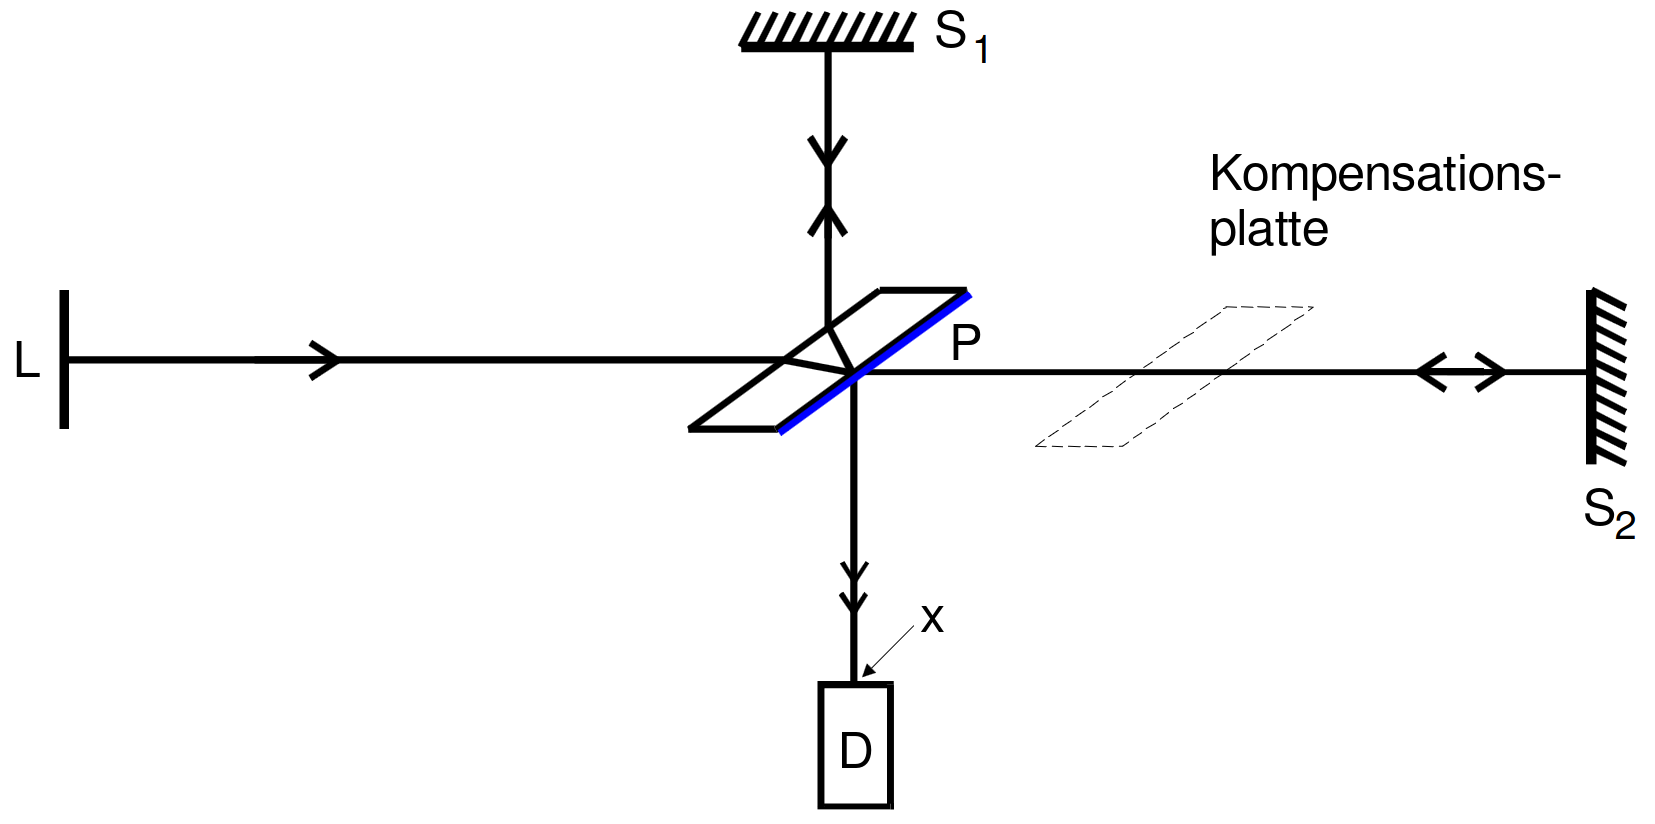
\includegraphics[width=0.8\textwidth]{img/aufbau.png}
    \caption{Aufbau des Michelson-Interferometers \cite{V401}.}
    \label{fig:Aufbau}
\end{figure}

Der schematische Aufbau des Michelson-Interferometers ist in Abbildung \ref{fig:Aufbau} zu sehen.
Er besteht aus einem Laser, einem semipermeablen Spiegel als Strahlteiler, zwei Spiegeln und einem Lichtdetektor.
Der Spiegel $\text{S}_1$ ist auf einem Mikrometerschraubstock montiert, mit dem sich die Position des Spiegels verändern lässt.
Die Mikrometerschraube wird mit einem Motor angetrieben. Zwischen dem Strahlteiler und dem Spiegel $\text{S}_1$ befindet sich
eine Kammer die evakuiert werden kann, um den Brechungsindex zu verändern. 
Zwischen dem Strahlteiler und dem Spiegel $\text{S}_2$ befindet sich eine Kompensationsplatte.
Der Lichtdetektor ist an einen Verstärker angeschlossen, der die Signale an einen Zähler weiterleitet.
Es wird die Anzahl der Wechsel zwischen Minima und Maxima gezählt.

\subsection{Messung}

Zunächst wird der Laser eingeschaltet und die Position des Spiegels $\text{S}_1$ so eingestellt, dass das Interferenzmuster
scharf zu erkennen ist. Die Linien des Interferenzmusters sollen wagerecht verlaufen.
\\
\\
Im ersten Versuchsabschnitt wird die Wellenlänge des Lasers bestimmt. Dazu wird die Anzahl der Interferenzmaxima gezählt, die
entstehen, wenn der Spiegel $\text{S}_1$ um $\SI{5}{\milli\meter}$ verschoben wird. Der Motor wird auf Geschwindigkeit $2$ eingestellt.
Die Messung wird von der $\SI{5}{\milli\meter}$  bis zur $\SI{10}{\milli\meter}$ Markierung der Schraube durchgeführt.
Die Anzahl der Maxima wird in beide Verschiebungsrichtungen je fünf mal gemessen. Nach jeder Messung wird der Zähler zurückgesetzt.
\\
\\
Im zweiten Versuchsabschnitt wird der Brechungsindex von Luft bestimmt. 
Dazu wird die Kammer zwischen dem semipermeablen Spiegel und dem Spiegel $\text{S}_1$ evakuiert.
Die Kammer wird auf einen Unterdruck von $\SI{-0.8}{\bar}$ gebracht.
Es wird die Anzahl der Interferenzmaxima gezählt, die entstehen, wenn die Kammer evakuiert wird. 
Seperat wird die Anzahl der Maxima aufgenommen, die zustande kommen wenn sie wieder mit Luft gefüllt wird.
Die Messung wird wieder je fünf mal durchgeführt. Nach jeder Messung wird der Zähler zurückgesetzt.